%=============================================================
% Session 03 – The Perceptron
% Deep Learning Course – IIIT Dharwad
% Instructors: Prof. S R M Prasanna & Dr. Sunil Saumya
%=============================================================
\documentclass[12pt,a4paper]{article}

%-------------------------------------------------------------
% Packages
%-------------------------------------------------------------
\usepackage{amsmath,amsthm,amssymb,mathtools}
\usepackage{tikz}
\usetikzlibrary{arrows.meta,positioning,shapes.geometric,calc,fit,backgrounds}
\usepackage{graphicx}
\usepackage{booktabs,tabularx,multirow}
\usepackage[ruled,vlined,linesnumbered]{algorithm2e}
\usepackage[most]{tcolorbox}
\usepackage{hyperref}
\usepackage[capitalize,noabbrev]{cleveref}
\usepackage[margin=1in]{geometry}
\usepackage{fancyhdr}
\usepackage{enumitem}
\usepackage{xcolor}
\usepackage{listings}
\usepackage{microtype}
\usepackage{parskip}

%-------------------------------------------------------------
% Colours
%-------------------------------------------------------------
\definecolor{codeblue}{RGB}{0,90,160}
\definecolor{codegray}{RGB}{100,100,100}
\definecolor{codered}{RGB}{180,30,30}
\definecolor{codecomment}{RGB}{80,130,80}

%-------------------------------------------------------------
% Listings (Python)
%-------------------------------------------------------------
\lstdefinestyle{python}{
  language=Python,
  basicstyle=\ttfamily\small,
  keywordstyle=\color{codeblue}\bfseries,
  commentstyle=\color{codecomment}\itshape,
  stringstyle=\color{codered},
  numberstyle=\tiny\color{codegray},
  numbers=left,
  numbersep=8pt,
  breaklines=true,
  frame=single,
  framerule=0.4pt,
  rulecolor=\color{gray!60},
  backgroundcolor=\color{gray!5},
  showstringspaces=false,
  tabsize=4,
}

%-------------------------------------------------------------
% tcolorbox environments
%-------------------------------------------------------------
\newtcolorbox{keyinsight}[1][]{colback=blue!5!white,colframe=blue!75!black,
  fonttitle=\bfseries,title=Key Insight,#1}
\newtcolorbox{example}[1][]{colback=green!5!white,colframe=green!75!black,
  fonttitle=\bfseries,title=Example,#1}
\newtcolorbox{warningbox}[1][]{colback=red!5!white,colframe=red!75!black,
  fonttitle=\bfseries,title=Warning,#1}

%-------------------------------------------------------------
% amsthm environments
%-------------------------------------------------------------
\newtheorem{theorem}{Theorem}[section]
\newtheorem{lemma}[theorem]{Lemma}
\newtheorem{definition}{Definition}[section]
\newtheorem{remark}{Remark}[section]

%-------------------------------------------------------------
% Header / Footer
%-------------------------------------------------------------
\pagestyle{fancy}
\fancyhf{}
\fancyhead[L]{\small Deep Learning -- Session 03}
\fancyhead[R]{\small The Perceptron}
\fancyfoot[C]{\thepage}
\renewcommand{\headrulewidth}{0.4pt}

%-------------------------------------------------------------
% Hyperref setup
%-------------------------------------------------------------
\hypersetup{
  colorlinks=true,
  linkcolor=blue!70!black,
  urlcolor=blue!70!black,
  citecolor=green!50!black,
  pdftitle={Session 03 -- The Perceptron},
  pdfauthor={IIIT Dharwad Deep Learning Course},
}

%-------------------------------------------------------------
% Convenience macros
%-------------------------------------------------------------
\newcommand{\vect}[1]{\mathbf{#1}}
\newcommand{\sgn}{\operatorname{sgn}}
\newcommand{\step}{\operatorname{step}}
\newcommand{\R}{\mathbb{R}}

%=============================================================
\begin{document}
%=============================================================

%-------------------------------------------------------------
% Title Page
%-------------------------------------------------------------
\begin{titlepage}
  \centering
  \vspace*{2cm}

  {\Huge\bfseries Deep Learning\par}
  \vspace{0.4cm}
  {\Large\bfseries Session 03 Lecture Notes\par}
  \vspace{1.2cm}

  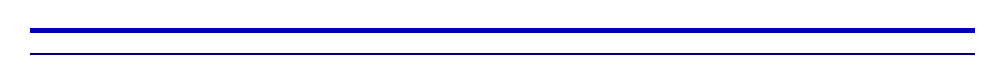
\begin{tikzpicture}
    \draw[blue!70!black, line width=2pt] (0,0) -- (12,0);
    \draw[blue!40!black, line width=0.8pt] (0,-0.3) -- (12,-0.3);
  \end{tikzpicture}

  \vspace{1.0cm}
  {\LARGE\bfseries The Perceptron:\par}
  \vspace{0.3cm}
  {\large From Biological Neurons to Multilayer Networks\par}
  \vspace{1.5cm}

  \begin{tabular}{ll}
    \textbf{Topic:}       & Biological Neurons $\to$ McCulloch-Pitts Model $\to$
                            Perceptron $\to$ MLP \\[4pt]
    \textbf{Session:}     & 03 \\[4pt]
    \textbf{Duration:}    & 1 hour 26 minutes 48 seconds \\[4pt]
    \textbf{Instructors:} & Prof.\ S~R~M~Prasanna \& Dr.\ Sunil Saumya \\[4pt]
    \textbf{Institute:}   & IIIT Dharwad \\[4pt]
    \textbf{Slide Decks:} & \texttt{02-DL-NNIntro} (slides 13--18)
                            \& \texttt{03-DL-Perceptron} (slides 5--14) \\[4pt]
    \textbf{Video:}       & \url{https://vimeo.com/1140267865} \\
  \end{tabular}

  \vspace{2cm}

  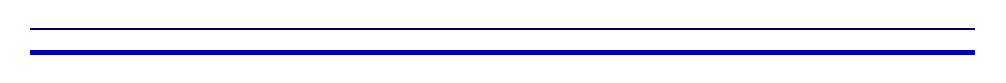
\begin{tikzpicture}
    \draw[blue!70!black, line width=2pt] (0,0) -- (12,0);
    \draw[blue!40!black, line width=0.8pt] (0,0.3) -- (12,0.3);
  \end{tikzpicture}

  \vfill
  {\small These notes synthesise the lecture transcript and visual extractions.
  They are intended as a study companion, not a replacement for the original lecture.}
\end{titlepage}

%-------------------------------------------------------------
% Table of Contents
%-------------------------------------------------------------
\tableofcontents
\newpage

%=============================================================
\section{Introduction}
\label{sec:intro}
%=============================================================

Session~03 forms the conceptual bridge between biological inspiration
and practical, trainable machine-learning models.
The session opens with a focused recap of how the human brain motivates
the neural-network paradigm, then introduces the first two mathematical
neuron models -- the McCulloch--Pitts (MP) neuron and Rosenblatt's
Perceptron -- before demonstrating the Perceptron learning algorithm
on a concrete placement-prediction dataset implemented live in PyTorch.
The session closes by analysing the Perceptron's inherent limitations
and motivating the transition to multilayer perceptrons (MLPs).

\subsection*{Session roadmap}

\begin{enumerate}[label=\textbf{\arabic*.}]
  \item Biological-to-artificial neuron motivation (recap)
  \item McCulloch--Pitts (MP) model -- fixed weights, no learning
  \item Activation dynamics versus synaptic dynamics
  \item Learning laws -- the general weight-update principle
  \item Rosenblatt's Perceptron -- error-driven weight updates
  \item Perceptron working examples (with and without bias)
  \item Perceptron Trick -- learning a decision boundary
  \item PyTorch implementation and visualisation
  \item Perceptron Representation Problem -- XOR, linear inseparability
  \item Beyond the single-layer perceptron -- MLPs
\end{enumerate}

\begin{keyinsight}[title=The Key Question of This Session]
A single biological neuron performs only a simple weighted sum followed
by a threshold comparison.
\emph{Where does the power of a neural network come from?}
The answer lies not in the individual unit but in the organisation:
billions of such units arranged in \textbf{layers} of interconnected
neurons, mirroring the layered architecture of the human cortex.
\end{keyinsight}

%=============================================================
\section{Background and Prerequisites}
\label{sec:background}
%=============================================================

\subsection{The Biological Neuron}
\label{subsec:bio-neuron}

The biological neuron consists of three primary functional parts:
\begin{itemize}
  \item \textbf{Dendrites} -- input channels that receive electrochemical
        signals from neighbouring neurons.
  \item \textbf{Cell body (soma)} -- acts as a summing junction,
        integrating all incoming potentials.
  \item \textbf{Axon and synaptic junctions} -- output channel; the
        junction strength (synaptic weight) encodes learned knowledge.
\end{itemize}

\begin{definition}[Synaptic Plasticity]
\label{def:plasticity}
The strength of a synaptic junction is not fixed.
Junctions that are \emph{repeatedly triggered} grow stronger; those
used infrequently gradually weaken.
This continuous self-modification is called \textbf{synaptic plasticity}
and is the biological basis for learning and memory.
\end{definition}

From the instructor's lecture:
\begin{quote}
``The synaptic junction is mimicked in the artificial neuron as what
are called weight parameters. In increasing large amount of data,
we learn the parameters representing these junction strengths.''
\end{quote}

\subsection{From Biology to Computation}
\label{subsec:bio-to-comp}

\Cref{tab:bio-artificial} summarises the mapping from biological structures
to their artificial counterparts.

\begin{table}[ht]
\centering
\caption{Biological neuron versus artificial neuron correspondence}
\label{tab:bio-artificial}
\begin{tabular}{lll}
\toprule
\textbf{Biological Structure} & \textbf{Artificial Analogue} & \textbf{Role} \\
\midrule
Dendrites             & Input connections $a_i$          & Receive signals \\
Synaptic junction     & Weight parameter $w_i$           & Store learned knowledge \\
Cell body (soma)      & Summation node $\sum w_i a_i$    & Integrate inputs \\
Resting potential     & Bias term $\theta$ (or $b$)      & Set firing threshold \\
Axon hillock          & Activation function $f(\cdot)$   & Non-linear gating \\
Axon output           & Output signal $s = f(x)$         & Forward signal \\
Plasticity            & Weight update rule $\Delta w_i$  & Learning \\
\bottomrule
\end{tabular}
\end{table}

\subsection{Activation Dynamics vs.\ Synaptic Dynamics}
\label{subsec:dynamics}

Two distinct types of temporal evolution govern a neural network:

\begin{description}
  \item[Activation dynamics] How the \emph{activation values} of neurons
        change as a function of time during inference (the forward pass).
  \item[Synaptic dynamics] How the \emph{weight parameters} change as a
        function of time during training (the learning process).
\end{description}

\begin{remark}
\label{rem:learning-concept}
In the context of neural networks, \emph{learning} is precisely the
process of adjusting weight parameters.
A learning law specifies \emph{how} the adjustment $\Delta w_i(t)$
is computed at each training step.
\end{remark}

%=============================================================
\section{The McCulloch--Pitts Neuron Model}
\label{sec:mp-model}
%=============================================================

\subsection{Mathematical Formulation}
\label{subsec:mp-math}

The McCulloch--Pitts (MP) model, proposed in 1943, was the first
published mathematical model of an artificial neuron.
It introduced the fundamental two-stage computation that underlies
all subsequent neural-network models.

\begin{definition}[MP Neuron]
\label{def:mp-neuron}
Given $M$ inputs $a_1, a_2, \ldots, a_M$ with associated weights
$w_1, w_2, \ldots, w_M$ and a bias (threshold) $\theta$, the MP neuron
computes:
\begin{align}
  x &= \sum_{i=1}^{M} w_i\, a_i - \theta \label{eq:activation}\\
  s &= f(x) \label{eq:output}
\end{align}
where $x$ is the \textbf{activation value} and $s$ is the \textbf{output value}.
\end{definition}

The function $f(\cdot)$ in \cref{eq:output} is typically a non-linear
(binary) function.
Two common choices are the \emph{step function} and the \emph{sign function}:

\begin{align}
  \step(x) &= \begin{cases} 1 & \text{if } x > 0 \\ 0 & \text{if } x \leq 0 \end{cases}
  \label{eq:step}\\[6pt]
  \sgn(x)  &= \begin{cases} +1 & \text{if } x > 0 \\ -1 & \text{if } x < 0 \\ 0 & \text{if } x = 0 \end{cases}
  \label{eq:sign}
\end{align}

\subsection{Architecture Diagram}
\label{subsec:mp-diagram}

\Cref{fig:mp-neuron} illustrates the MP neuron's architecture.

\begin{figure}[ht]
\centering
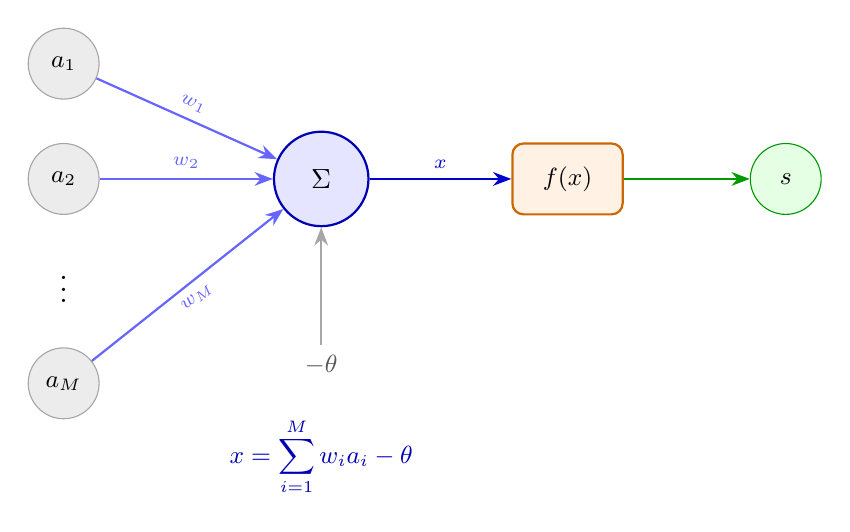
\begin{tikzpicture}[
  node distance=0.8cm and 1.6cm,
  inputnode/.style={circle, draw=gray!70, fill=gray!15, minimum size=0.9cm, font=\small},
  sumnode/.style={circle, draw=blue!70!black, fill=blue!10, minimum size=1.2cm,
                  font=\normalsize, thick},
  actnode/.style={rectangle, rounded corners=4pt, draw=orange!80!black,
                  fill=orange!10, minimum width=1.4cm, minimum height=0.9cm,
                  font=\small, thick},
  outnode/.style={circle, draw=green!60!black, fill=green!10,
                  minimum size=0.9cm, font=\small},
  >=Stealth
]

% Input nodes
\node[inputnode] (a1) {$a_1$};
\node[inputnode, below=0.55cm of a1] (a2) {$a_2$};
\node[below=0.45cm of a2, font=\large] (dots) {$\vdots$};
\node[inputnode, below=0.45cm of dots] (am) {$a_M$};

% Summation node
\node[sumnode, right=2.2cm of a2] (sum) {$\Sigma$};

% Activation node
\node[actnode, right=1.8cm of sum] (act) {$f(x)$};

% Output
\node[outnode, right=1.6cm of act] (out) {$s$};

% Bias
\node[below=1.5cm of sum, font=\small, text=gray!70!black] (bias) {$-\theta$};

% Arrows: inputs to sum
\draw[->, thick, blue!60] (a1) -- node[above, sloped, font=\scriptsize] {$w_1$} (sum);
\draw[->, thick, blue!60] (a2) -- node[above, sloped, font=\scriptsize] {$w_2$} (sum);
\draw[->, thick, blue!60] (am) -- node[below, sloped, font=\scriptsize] {$w_M$} (sum);

% Bias arrow
\draw[->, thick, gray!70] (bias) -- (sum);

% Sum to activation
\draw[->, thick, blue!80!black] (sum) -- node[above, font=\scriptsize] {$x$} (act);

% Activation to output
\draw[->, thick, green!60!black] (act) -- (out);

% Label the summation equation below the figure
\node[below=2.3cm of sum, font=\small, text=blue!70!black]
  {$x = \displaystyle\sum_{i=1}^{M} w_i a_i - \theta$};

\end{tikzpicture}
\caption{McCulloch--Pitts neuron model.
         $M$ weighted inputs are summed and the bias $\theta$ is subtracted
         to form the activation value $x$, which is then passed through a
         non-linear output function $f(\cdot)$ to produce the output $s$.}
\label{fig:mp-neuron}
\end{figure}

\subsection{Limitations of the MP Model}
\label{subsec:mp-limits}

\begin{warningbox}[title=Critical Limitation of the MP Model]
The MP model assumes \textbf{fixed weights}.
There is no mechanism for the model to \emph{learn} the weight values
from data.
Weights must be computed or assigned manually before use -- a serious
practical obstacle when the number of inputs and neurons grows large.
\end{warningbox}

This limitation motivated Rosenblatt's seminal advance: a model that
\emph{automatically adjusts} its weights in response to prediction
errors, introducing \emph{learning} into the computational neuron.

%=============================================================
\section{Learning Laws and the Perceptron}
\label{sec:perceptron}
%=============================================================

\subsection{The General Weight-Update Principle}
\label{subsec:weight-update}

All neural-network learning algorithms share a common skeleton:
at time step $t$, compute an incremental change $\Delta w_i(t)$ and
add it to the current weight:

\begin{equation}
  w_i(t+1) = w_i(t) + \Delta w_i(t)
  \label{eq:weight-update}
\end{equation}

The specific rule for computing $\Delta w_i(t)$ defines the
\emph{learning law}.
Common examples include: Hebb's law, the Perceptron learning law,
the Delta (Widrow--Hoff LMS) law, the correlation law, and the
instar/outstar laws.

\subsection{Rosenblatt's Perceptron Model}
\label{subsec:perceptron-model}

Frank Rosenblatt (1958) introduced the Perceptron as the first model
that could \emph{automatically learn} its weight parameters from labelled
examples.
The architecture retains the MP neuron equations (\cref{eq:activation,eq:output})
but adds an error-driven weight-update rule.

\begin{definition}[Perceptron Learning Rule]
\label{def:perceptron-rule}
Given a target output $b$ and actual output $s = f(x)$, define the
\textbf{error signal}:
\begin{equation}
  \delta = b - s
  \label{eq:error}
\end{equation}
The weight update for the $i$-th input connection is:
\begin{equation}
  \Delta w_i = \eta\,\delta\,a_i
  \label{eq:delta-w}
\end{equation}
where $\eta > 0$ is the \textbf{learning rate}.
The updated weight is:
\begin{equation}
  w_i(t+1) = w_i(t) + \eta\,\delta\,a_i
  \label{eq:update-rule}
\end{equation}
\end{definition}

\subsubsection{Effect of the Error Signal}
\label{subsubsec:error-effect}

\Cref{tab:error-cases} shows the three possible cases for $\delta$ and
the resulting effect on the weights.

\begin{table}[ht]
\centering
\caption{Perceptron weight-update cases based on the error $\delta = b - s$}
\label{tab:error-cases}
\begin{tabular}{cccp{6.5cm}}
\toprule
\textbf{Actual} $s$ & \textbf{Target} $b$ & $\delta$ & \textbf{Effect on weights} \\
\midrule
$s = b$  & --  & $0$  & No update; current weights are correct for this sample \\
$0$      & $1$ & $+1$ & Increase weights connected to active inputs (push activation up) \\
$1$      & $0$ & $-1$ & Decrease weights connected to active inputs (push activation down) \\
\bottomrule
\end{tabular}
\end{table}

\subsection{The Discrete Perceptron Learning Law}
\label{subsec:discrete-perceptron}

In the formal statement used in the course slides, the Perceptron
learning law is written using the sign function:

\begin{align}
  \Delta w_i &= \eta\bigl[b_i - \sgn(\vect{w}_i^T \vect{a})\bigr]\,a
  \label{eq:discrete-law-1}\\
  \Delta w_{ij} &= \eta\bigl[b_j - \sgn(\vect{w}_i^T \vect{a})\bigr]\,a_j,
    \quad j = 1, 2, \ldots, M
  \label{eq:discrete-law-2}
\end{align}

Key properties of the Perceptron learning law:
\begin{itemize}
  \item Weights are adjusted \emph{only} when the actual output $s_j$
        is incorrect.
  \item Weights are initialised to small random values prior to learning.
  \item It is a \textbf{supervised learning} algorithm: it requires a
        desired (target) output for each input.
  \item \textbf{Weights converge to final values by repeated use of
        input--output pairs.}
  \item The learning rate $\eta \ll 1$ is kept small to ensure stable
        error-corrective updates.
\end{itemize}

\begin{keyinsight}[title=The Breakthrough of Learning]
Before Rosenblatt's Perceptron, weights were fixed and had to be set
manually.
The Perceptron demonstrated for the first time that a neural unit could
\emph{automatically learn} its weights from data.
This was a foundational result in the history of artificial intelligence.
From the lecture: ``The concept of learning was demonstrated for the
first time in the neural network history. That's why this is treated as
one of the breakthrough results.''
\end{keyinsight}

%=============================================================
\section{Perceptron Working: Numerical Examples}
\label{sec:perceptron-examples}
%=============================================================

\subsection{Forward Pass Without Bias}
\label{subsec:no-bias}

Consider a three-input perceptron with the following values:

\begin{center}
\begin{tabular}{llll}
\toprule
\textbf{Input} & $x_1 = 0.2$ & $x_2 = 0.4$ & $x_3 = 0.6$ \\
\textbf{Weight} & $w_1 = -0.3$ & $w_2 = 0.4$ & $w_3 = -0.8$ \\
\bottomrule
\end{tabular}
\end{center}

The weighted sum is:
\begin{align}
  \sum_{i=1}^{3} w_i x_i
    &= (0.2)(-0.3) + (0.4)(0.4) + (0.6)(-0.8) \notag \\
    &= -0.06 + 0.16 - 0.48 \notag \\
    &= -0.38
  \label{eq:ws-no-bias}
\end{align}

Applying the step function: $f(-0.38) = \mathbf{0}$, since $-0.38 \leq 0$.

\subsection{Forward Pass With Bias}
\label{subsec:with-bias}

Using the same inputs and weights but adding a bias $b = 0.5$:
\begin{align}
  \sum_{i=1}^{3} w_i x_i + b
    &= -0.38 + 0.5 \notag \\
    &= 0.12
  \label{eq:ws-bias}
\end{align}

Applying the step function: $f(0.12) = \mathbf{1}$, since $0.12 > 0$.

\begin{example}[title=Impact of the Bias Term]
Adding a bias of $b = 0.5$ flipped the output from $0$ to $1$.
The bias acts as a learnable threshold that shifts the decision boundary
away from the origin.
\textbf{Without bias, the decision boundary must pass through the origin},
severely restricting which patterns can be classified correctly.
\end{example}

\subsection{Perceptron Architecture Diagram (With Bias)}
\label{subsec:perceptron-arch-diagram}

\begin{figure}[ht]
\centering
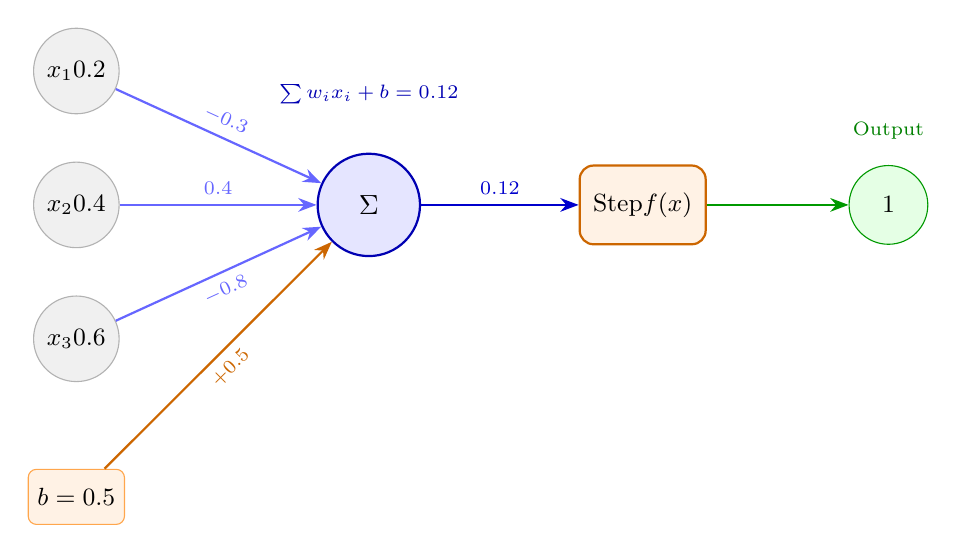
\begin{tikzpicture}[
  node distance=0.9cm and 2.0cm,
  inputnode/.style={circle, draw=gray!60, fill=gray!12, minimum size=1.0cm, font=\small},
  biasnode/.style={rectangle, rounded corners=3pt, draw=orange!70, fill=orange!10,
                   minimum width=1.1cm, minimum height=0.7cm, font=\small},
  sumnode/.style={circle, draw=blue!70!black, fill=blue!10, minimum size=1.3cm,
                  font=\normalsize, thick},
  actnode/.style={rectangle, rounded corners=5pt, draw=orange!80!black,
                  fill=orange!10, minimum width=1.6cm, minimum height=1.0cm,
                  font=\small, thick},
  outnode/.style={circle, draw=green!60!black, fill=green!10,
                  minimum size=1.0cm, font=\small\bfseries},
  >=Stealth
]

% Input nodes
\node[inputnode] (x1) {$x_1$\\$0.2$};
\node[inputnode, below=0.6cm of x1] (x2) {$x_2$\\$0.4$};
\node[inputnode, below=0.6cm of x2] (x3) {$x_3$\\$0.6$};

% Bias node
\node[biasnode, below=1.1cm of x3] (bias) {$b=0.5$};

% Summation node
\node[sumnode, right=2.5cm of x2] (sum) {$\Sigma$};

% Activation function node
\node[actnode, right=2.0cm of sum] (act) {Step\\$f(x)$};

% Output node
\node[outnode, right=1.8cm of act] (out) {$1$};

% Arrows
\draw[->, thick, blue!60] (x1) -- node[above, sloped, font=\scriptsize] {$-0.3$} (sum);
\draw[->, thick, blue!60] (x2) -- node[above, font=\scriptsize] {$0.4$} (sum);
\draw[->, thick, blue!60] (x3) -- node[below, sloped, font=\scriptsize] {$-0.8$} (sum);
\draw[->, thick, orange!80!black] (bias) -- node[below, sloped, font=\scriptsize] {$+0.5$} (sum);
\draw[->, thick, blue!80!black] (sum) -- node[above, font=\scriptsize] {$0.12$} (act);
\draw[->, thick, green!60!black] (act) -- (out);

% Annotation
\node[above=0.2cm of out, font=\scriptsize, text=green!50!black] {Output};
\node[above=0.5cm of sum, font=\scriptsize, text=blue!70!black] {$\sum w_i x_i + b = 0.12$};

\end{tikzpicture}
\caption{Perceptron with bias.
         The three weighted inputs sum to $-0.38$; adding bias $b=0.5$ gives
         $0.12$, which crosses the threshold to produce output $1$.}
\label{fig:perceptron-bias}
\end{figure}

\subsection{PyTorch Implementation}
\label{subsec:pytorch-impl}

The following PyTorch code (demonstrated live in Google Colab during
the session) replicates both forward-pass computations:

\begin{lstlisting}[style=python, caption={Perceptron forward pass in PyTorch (V13 -- 00:30:00)}, label={lst:forward-pass}]
import torch

# Inputs and weights
x = torch.tensor([0.2, 0.4, 0.6])
weights = torch.tensor([-0.3, 0.4, -0.8])

# Weighted sum (no bias)
weighted_sum = torch.dot(weights, x)   # tensor(-0.3800)

# Step activation function
def step_function(z):
    return 1 if z >= 0 else 0

output = step_function(weighted_sum)              # 0

# With bias b = 0.5
bias = 0.5
output_with_bias = step_function(weighted_sum + bias)  # 1
print(f"Without bias: {output}")         # 0
print(f"With bias:    {output_with_bias}")  # 1
\end{lstlisting}

%=============================================================
\section{Learning a Decision Boundary -- The Perceptron Trick}
\label{sec:decision-boundary}
%=============================================================

\subsection{Problem Setup: Placement Prediction}
\label{subsec:placement-problem}

The session uses a toy placement-prediction dataset to motivate the
Perceptron Trick.
Each student is described by two features -- CGPA ($x_1$) and IQ
($x_2$, scaled to IQ/10) -- and labelled with a binary placement
outcome ($y \in \{0, 1\}$).

\begin{table}[ht]
\centering
\caption{Placement dataset used in the Perceptron Trick demonstration}
\label{tab:placement}
\begin{tabular}{cccc}
\toprule
\textbf{Student} & \textbf{CGPA} ($x_1$) & \textbf{IQ/10} ($x_2$) & \textbf{Placed?} ($y$) \\
\midrule
1 & 6.5  & 11.0 & 0 (Not placed) \\
2 & 7.2  & 12.0 & 1 (Placed) \\
3 & 8.0  & 10.5 & 1 (Placed) \\
\bottomrule
\end{tabular}
\end{table}

\subsection{The Decision Boundary Equation}
\label{subsec:db-equation}

A perceptron with bias weight $w_0$ and feature weights $w_1, w_2$
classifies a point $(x_1, x_2)$ by the sign of:
\begin{equation}
  z = w_0 x_0 + w_1 x_1 + w_2 x_2, \qquad x_0 = 1 \text{ (bias input)}
  \label{eq:linear-combination}
\end{equation}

The \textbf{decision boundary} is the set of points where $z = 0$:
\begin{equation}
  w_0 + w_1 x_1 + w_2 x_2 = 0
  \label{eq:decision-boundary}
\end{equation}

Solving for $x_2$ gives the boundary line in feature space:
\begin{equation}
  x_2 = -\frac{w_0 + w_1 x_1}{w_2}
  \label{eq:boundary-line}
\end{equation}

\subsection{Numerical Derivation with Initial Weights}
\label{subsec:numerical-db}

Starting with random initial weights $w_0 = -1,\ w_1 = 0.5,\ w_2 = -0.3$:

\begin{align}
  -1 + 0.5\,x_1 - 0.3\,x_2 &= 0 \notag \\
  -0.3\,x_2 &= 1 - 0.5\,x_1 \notag \\
  x_2 &= \frac{1 - 0.5\,x_1}{-0.3} \notag \\
  x_2 &= -3.333 + 1.6\overline{6}\,x_1
  \label{eq:initial-boundary}
\end{align}

\begin{keyinsight}[title=Geometric Interpretation]
The decision boundary in \cref{eq:decision-boundary} is a hyperplane
in the $M$-dimensional feature space.
In two dimensions it is a straight line.
Points on one side are predicted as class 1; points on the other side
as class 0.
The Perceptron Trick iteratively rotates and translates this line until
all training points are correctly classified.
\end{keyinsight}

\subsection{The Perceptron Trick Algorithm}
\label{subsec:perceptron-trick}

The key intuition is: if a point is \emph{misclassified}, adjust the
weights so that the decision boundary moves towards the misclassified
point.

\begin{algorithm}[H]
\caption{Perceptron Learning (Perceptron Trick)}
\label{alg:perceptron-trick}
\SetAlgoLined
\DontPrintSemicolon
\KwIn{Training set $\{(\vect{x}^{(k)}, y^{(k)})\}_{k=1}^{N}$,
      learning rate $\eta$, max epochs $T$}
\KwOut{Weight vector $\vect{w} = (w_0, w_1, \ldots, w_n)^T$}
\BlankLine

\textbf{Initialise:} Set $x_0 \leftarrow 1$ (bias input)\;
\textbf{Initialise:} $w_i \leftarrow$ small random values, $i = 0, 1, \ldots, n$\;
\BlankLine

\For{$\text{epoch} = 1$ \KwTo $T$}{
  \For{each training example $(\vect{x}^{(k)}, y^{(k)})$}{
    Compute weighted sum: $z \leftarrow \sum_{i=0}^{n} w_i x_i^{(k)}$\;
    \BlankLine
    Predict output:
    $\hat{y} \leftarrow \begin{cases} 1 & \text{if } z \geq 0 \\ 0 & \text{if } z < 0 \end{cases}$\;
    \BlankLine
    Compute error: $e \leftarrow y^{(k)} - \hat{y}$\;
    \BlankLine
    \If{$e \neq 0$ \textup{(misclassification)}}{
      \For{$i = 0, 1, \ldots, n$}{
        $w_i \leftarrow w_i + \eta \cdot e \cdot x_i^{(k)}$
        \tcp*{Shift boundary toward point}
      }
    }
  }
  \BlankLine
  \lIf{no misclassified points}{\textbf{break}}
}
\Return $\vect{w}$\;
\end{algorithm}

\subsection{Decision Boundary Evolution Diagram}
\label{subsec:db-evolution}

\Cref{fig:db-evolution} illustrates how the decision boundary rotates
across training epochs on the placement dataset.

\begin{figure}[ht]
\centering
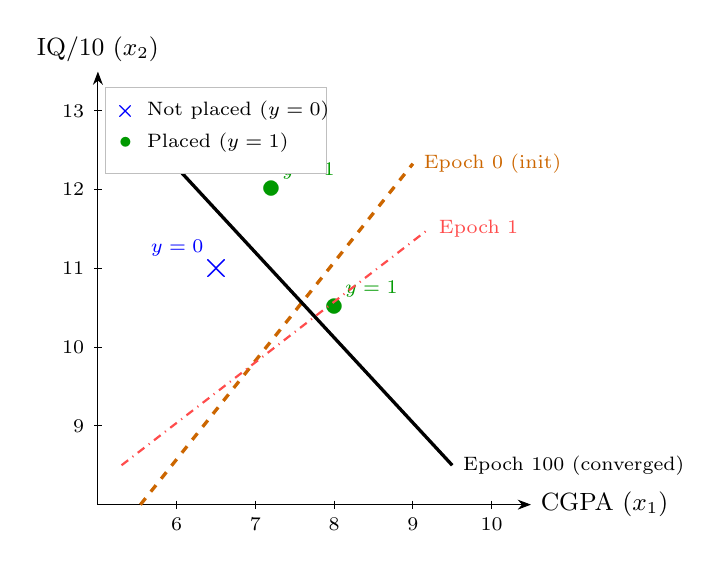
\begin{tikzpicture}[scale=1.0, >=Stealth]

% Axes
\draw[->] (0,0) -- (5.5,0) node[right, font=\small] {CGPA ($x_1$)};
\draw[->] (0,0) -- (0,5.5) node[above, font=\small] {IQ/10 ($x_2$)};

% Axis ticks and labels
\foreach \x/\xl in {1/6,2/7,3/8,4/9,5/10}{
  \draw (\x,0.05) -- (\x,-0.05) node[below, font=\scriptsize] {\xl};
}
\foreach \y/\yl in {1/9,2/10,3/11,4/12,5/13}{
  \draw (0.05,\y) -- (-0.05,\y) node[left, font=\scriptsize] {\yl};
}

% Class-0 point: CGPA=6.5 -> x=1.5, IQ/10=11.0 -> y=3.0
\node[blue, font=\Large] at (1.5,3.0) {\texttimes};
\node[blue, font=\scriptsize, above left=0.05cm] at (1.5,3.0) {$y=0$};

% Class-1 points: CGPA=7.2 -> x=2.2, IQ/10=12.0 -> y=4.0
\node[green!60!black, font=\Large] at (2.2,4.0) {$\bullet$};
\node[green!60!black, font=\scriptsize, above right=0.02cm] at (2.2,4.0) {$y=1$};

% CGPA=8.0 -> x=3.0, IQ/10=10.5 -> y=2.5
\node[green!60!black, font=\Large] at (3.0,2.5) {$\bullet$};
\node[green!60!black, font=\scriptsize, above right=0.02cm] at (3.0,2.5) {$y=1$};

% Initial decision boundary (epoch 0): x2 = -3.333 + 1.667*x1
% At x1=6 (plot-x=1): x2 = -3.333 + 10 = 6.667 (plot-y=6.667-9=-2.333) -- off plot
% Use parametric: x_plot = x1-6, y_plot = x2-9
% x2 = -3.333 + 1.667*x1; at x1=6: x2=6.667; at x1=10: x2=13.333
% plot-x=x1-6, plot-y=x2-9
% x1=6->plot_x=0, x2=6.667->plot_y=-2.33 (clamp to 0)
% x1=6.54->x2=9 so plot_x=0.54, plot_y=0
% x1=10->plot_x=4, plot_y=4.33
\draw[orange!80!black, dashed, very thick]
  (0.54,0) -- (4.0,4.33)
  node[right, font=\scriptsize, orange!80!black] {Epoch 0 (init)};

% Epoch 1 boundary: slightly shifted
\draw[red!70, dashdotted, thick]
  (0.3,0.5) -- (4.2,3.5)
  node[right, font=\scriptsize, red!70] {Epoch 1};

% Final boundary (epoch 100): separates class 0 from class 1
\draw[black, very thick]
  (0.8,4.5) -- (4.5,0.5)
  node[right, font=\scriptsize] {Epoch 100 (converged)};

% Legend box
\begin{scope}[shift={(0.1,4.2)}]
  \draw[fill=white, draw=gray!50] (0,0) rectangle (2.8,1.1);
  \node[blue, font=\small] at (0.25,0.8) {\texttimes};
  \node[font=\scriptsize, right] at (0.4,0.8) {Not placed ($y=0$)};
  \node[green!60!black, font=\small] at (0.25,0.4) {$\bullet$};
  \node[font=\scriptsize, right] at (0.4,0.4) {Placed ($y=1$)};
\end{scope}

\end{tikzpicture}
\caption{Decision boundary evolution on the placement dataset.
         The boundary starts randomly (dashed orange), shifts after epoch~1
         (dash-dotted red), and converges to a clean separator at epoch~100
         (solid black).}
\label{fig:db-evolution}
\end{figure}

\subsection{Full PyTorch Training Loop}
\label{subsec:training-loop}

\begin{lstlisting}[style=python, caption={Full perceptron training loop with weight history (V20 -- 01:01:00)}, label={lst:training-loop}]
import torch

# Dataset: CGPA (x1), IQ/10 (x2), placement label
X_raw = torch.tensor([
    [6.5, 11.0],
    [7.2, 12.0],
    [8.0, 10.5],
], dtype=torch.float32)
Y = torch.tensor([0, 1, 1], dtype=torch.float32)

# Augment with bias column x0 = 1
bias_col = torch.ones(X_raw.shape[0], 1)
X = torch.cat([bias_col, X_raw], dim=1)   # shape (3, 3)

# Random weight initialisation: w0=-1, w1=0.5, w2=-0.3
W = torch.tensor([-1.0, 0.5, -0.3])

def predict(x_vec, w_vec):
    z = torch.dot(w_vec, x_vec)
    return 1 if z >= 0 else 0

eta = 0.1
epochs = 100
weight_history = []

for epoch in range(epochs):
    for i in range(len(X)):
        xi  = X[i]
        yi  = Y[i].item()
        y_hat = predict(xi, W)
        error = yi - y_hat
        if error != 0:
            W = W + eta * error * xi
    weight_history.append(W.clone())

W_epoch1  = weight_history[0]
W_epoch2  = weight_history[1]
W_final   = weight_history[-1]
print(f"Final weights: {W_final}")
\end{lstlisting}

\subsection{Weight History Across Training}
\label{subsec:weight-history}

\Cref{tab:weight-history} summarises how the three weight parameters
evolve during training.

\begin{table}[ht]
\centering
\caption{Weight evolution during perceptron training on the placement dataset}
\label{tab:weight-history}
\begin{tabular}{lccc}
\toprule
\textbf{Epoch} & $w_0$ (bias) & $w_1$ (CGPA) & $w_2$ (IQ/10) \\
\midrule
Initialisation & $-1.0$  & $0.5$  & $-0.3$  \\
Epoch 1        & shifts after first misclassification & updated & updated \\
Epoch 2        & further shift & further shift & further shift \\
$\vdots$       & $\vdots$ & $\vdots$ & $\vdots$ \\
Epoch $\leq 100$ & converged & converged & converged \\
\bottomrule
\multicolumn{4}{l}{\small Note: exact values vary per random seed.
Pattern: rapid changes in early epochs, stabilises once all} \\
\multicolumn{4}{l}{\small training points are correctly classified.} \\
\end{tabular}
\end{table}

%=============================================================
\section{The Perceptron Convergence Theorem}
\label{sec:convergence}
%=============================================================

\begin{theorem}[Perceptron Convergence Theorem]
\label{thm:perceptron-convergence}
If the training data is \textbf{linearly separable}, the perceptron
learning algorithm is guaranteed to converge -- that is, to find a
weight vector $\vect{w}^*$ that correctly classifies all training
examples -- in a \textbf{finite} number of weight updates.
\end{theorem}

\begin{remark}
\label{rem:convergence-finite}
The convergence theorem provides an upper bound on the number of
misclassifications before convergence, which depends on the margin
(the distance from the closest point to the separating hyperplane)
and the norm of the input vectors.
Specifically, if there exists a weight vector $\vect{w}^*$ with
$\|\vect{w}^*\| = 1$ such that $y^{(k)}(\vect{w}^{*T}\vect{x}^{(k)}) \geq \gamma$
for all $k$, the number of mistakes is at most $R^2/\gamma^2$ where
$R = \max_k \|\vect{x}^{(k)}\|$.
\end{remark}

\begin{keyinsight}[title=What the Convergence Theorem Does Not Guarantee]
The theorem guarantees convergence \emph{only when the data is linearly
separable}.
For non-linearly-separable data (e.g., XOR), the algorithm will never
converge -- the weights oscillate indefinitely.
Moreover, even when the data is linearly separable, the converged
solution is not necessarily optimal: there can be \emph{infinitely
many} valid separating hyperplanes.
\end{keyinsight}

%=============================================================
\section{Perceptron Representation Problem}
\label{sec:representation}
%=============================================================

\subsection{Linear Separability}
\label{subsec:linear-separability}

A binary classification problem on inputs $\{0, 1\}^M$ is
\textbf{linearly separable} if there exists a hyperplane
$\vect{w}^T \vect{x} = 0$ such that all class-1 points lie on one
side and all class-0 points on the other.

For $M = 2$ binary inputs there are $2^{2^M} = 2^4 = 16$ distinct
Boolean functions.
Of these 16 functions, only \textbf{14 are linearly separable}.

\begin{example}[title=Linearly Separable Boolean Functions]
The following two-input functions are linearly separable:
AND, OR, NOT, NOR, NAND, and their combinations.
Each can be implemented by a single-layer perceptron.
\end{example}

\subsection{The XOR Problem}
\label{subsec:xor}

XOR (exclusive-or) is the canonical example of a \emph{non-linearly
separable} function.
\Cref{tab:xor-truth} shows the truth table.

\begin{table}[ht]
\centering
\caption{XOR truth table showing non-linear separability}
\label{tab:xor-truth}
\begin{tabular}{ccc}
\toprule
$A$ & $B$ & $A \oplus B$ \\
\midrule
0 & 0 & 0 \\
0 & 1 & 1 \\
1 & 0 & 1 \\
1 & 1 & 0 \\
\bottomrule
\end{tabular}
\end{table}

No single straight line can separate the output-1 points
$\{(0,1),\,(1,0)\}$ from the output-0 points $\{(0,0),\,(1,1)\}$
in the unit square.
XNOR (the complement of XOR) is equally non-separable.

\subsection{Hard Problems}
\label{subsec:hard-problems}

Problems that are not linearly separable are called \textbf{hard
problems} for a single-layer perceptron.

\begin{definition}[Hard Problem]
\label{def:hard-problem}
A pattern classification problem is called a \textbf{hard problem} if
it is not representable by a single-layer perceptron -- i.e., the
classes are not linearly separable, and the perceptron learning
algorithm will not converge on it.
\end{definition}

As the input dimensionality $M$ increases, the fraction of Boolean
functions that are linearly separable decreases rapidly.
This means the single-layer perceptron becomes increasingly limited
as problems grow in complexity.

\begin{warningbox}[title=Practical Implication]
Real-world data (images, speech, text) is almost never linearly
separable in the raw input space.
Relying solely on a single-layer perceptron for such tasks will result
in the algorithm failing to converge and producing poor classifiers.
A deeper architecture is required.
\end{warningbox}

%=============================================================
\section{Beyond the Perceptron: Multilayer Networks}
\label{sec:mlp}
%=============================================================

\subsection{Two-Layer Networks: Convex Regions}
\label{subsec:two-layer}

Adding a \emph{single hidden layer} to the perceptron allows the
network to form \textbf{convex decision regions}.

\begin{definition}[Convex Region]
\label{def:convex}
A region $\mathcal{R} \subseteq \R^M$ is \textbf{convex} if, for any
two points $\vect{p}, \vect{q} \in \mathcal{R}$, the entire line
segment $\lambda\vect{p} + (1-\lambda)\vect{q}$ for
$\lambda \in [0,1]$ lies within $\mathcal{R}$.
\end{definition}

Each hidden-layer unit contributes one half-space boundary.
The intersection of these half-spaces forms a convex region.
A two-layer network can therefore solve XOR by combining two
linear separators.

\subsection{Three-Layer Networks: Arbitrary Regions}
\label{subsec:three-layer}

A second hidden layer (three layers total) can form the
\textbf{union of convex regions}, thereby approximating
\emph{any} finite binary classification boundary.
The shape and size of the class regions depend on the number of
hidden units in each layer.

\subsection{Four-Layer Networks: Full Generality}
\label{subsec:four-layer}

A four-layer network (input + three layers of nonlinear units)
can perform \textbf{any complex pattern classification} task.
This is the Multilayer Perceptron (MLP), also called a
feedforward fully-connected network.

\subsection{Network Capability Summary}
\label{subsec:network-summary}

\Cref{tab:network-capability} and \cref{fig:mlp-progression} compare
the representational power of increasingly deep perceptron networks.

\begin{table}[ht]
\centering
\caption{Decision region capability as a function of network depth}
\label{tab:network-capability}
\begin{tabularx}{\textwidth}{lllX}
\toprule
\textbf{Network}         & \textbf{Hidden Layers} & \textbf{Decision Region} & \textbf{Example Problems} \\
\midrule
1-layer perceptron       & 0 & Hyperplane (linear only) & AND, OR, NOT \\
2-layer (1 hidden layer) & 1 & Convex region            & XOR, bounded convex shapes \\
3-layer (2 hidden layers)& 2 & Arbitrary (non-convex)   & Any finite binary task \\
4-layer (3 hidden layers)& 3 & Any complex pattern      & General classification \\
\bottomrule
\end{tabularx}
\end{table}

\begin{figure}[ht]
\centering
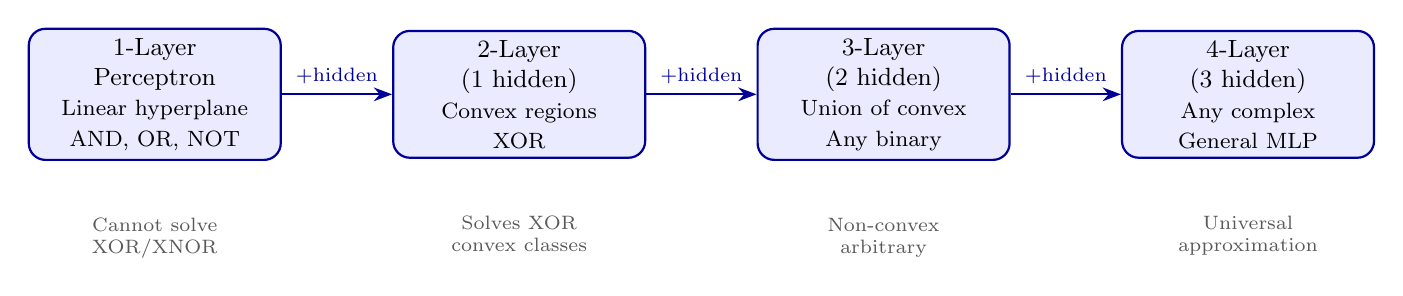
\begin{tikzpicture}[
  block/.style={rectangle, rounded corners=6pt, draw=blue!60!black,
                fill=blue!8, minimum width=3.2cm, minimum height=1.6cm,
                align=center, font=\small, thick},
  arrow/.style={->, thick, blue!60!black},
  label/.style={font=\scriptsize, text=gray!70!black, align=center},
  >=Stealth,
  node distance=1.2cm
]

\node[block] (L1) {1-Layer\\Perceptron\\{\footnotesize Linear hyperplane}\\{\footnotesize AND, OR, NOT}};
\node[block, right=1.4cm of L1] (L2) {2-Layer\\(1 hidden)\\{\footnotesize Convex regions}\\{\footnotesize XOR}};
\node[block, right=1.4cm of L2] (L3) {3-Layer\\(2 hidden)\\{\footnotesize Union of convex}\\{\footnotesize Any binary}};
\node[block, right=1.4cm of L3] (L4) {4-Layer\\(3 hidden)\\{\footnotesize Any complex}\\{\footnotesize General MLP}};

\draw[arrow] (L1) -- node[above, font=\scriptsize] {+hidden} (L2);
\draw[arrow] (L2) -- node[above, font=\scriptsize] {+hidden} (L3);
\draw[arrow] (L3) -- node[above, font=\scriptsize] {+hidden} (L4);

% Capability labels below
\node[label, below=0.6cm of L1] {Cannot solve\\XOR/XNOR};
\node[label, below=0.6cm of L2] {Solves XOR\\convex classes};
\node[label, below=0.6cm of L3] {Non-convex\\arbitrary};
\node[label, below=0.6cm of L4] {Universal\\approximation};

\end{tikzpicture}
\caption{Progression of representational power as hidden layers are added.
         Each additional layer unlocks a more expressive class of decision
         boundaries, culminating in the universal approximation capability
         of deep MLPs.}
\label{fig:mlp-progression}
\end{figure}

\subsection{The Problem of Multiple Solutions}
\label{subsec:multiple-solutions}

Even when the data is linearly separable, the Perceptron Trick finds
\emph{some} valid hyperplane -- but there may be infinitely many such
hyperplanes.
The algorithm has no notion of which separator is ``best.''
This motivates later techniques:

\begin{itemize}
  \item \textbf{Support Vector Machines} -- find the maximum-margin
        separator (widest possible gap between classes).
  \item \textbf{Backpropagation + gradient descent} -- optimise a
        smooth loss function over all weights simultaneously in MLPs.
\end{itemize}

\begin{keyinsight}[title=From Perceptron to Deep Learning]
The Perceptron established the foundational idea that neural units can
learn from data.
Its limitation -- inability to solve non-linearly-separable problems
-- directly motivated the development of multilayer networks.
These, combined with the backpropagation algorithm (introduced in later
sessions), form the basis of all modern deep learning systems.
\end{keyinsight}

%=============================================================
\section{Topology and Network Organisation}
\label{sec:topology}
%=============================================================

The term \textbf{topology} refers to how neurons are organised and
connected within a network.
Key design choices include:

\begin{enumerate}[label=(\alph*)]
  \item \textbf{Layer structure:} All neurons in a layer share the same
        activation dynamics and output function.
  \item \textbf{Connection type:}
        \begin{itemize}
          \item \emph{Interlayer connections} -- between adjacent layers
                (standard feedforward).
          \item \emph{Intralayer connections} -- within a layer
                (as in Hopfield networks).
          \item \emph{Both} -- recurrent networks.
        \end{itemize}
  \item \textbf{Information flow:}
        \begin{itemize}
          \item \emph{Feedforward} -- information flows from input to
                output only.
          \item \emph{Feedback (recurrent)} -- outputs feed back to
                earlier layers.
          \item \emph{Both} -- hybrid architectures.
        \end{itemize}
\end{enumerate}

\begin{remark}
\label{rem:power-of-layers}
The real power of neural networks does not come from the complexity
of individual neurons.
From the lecture: ``\ldots the strength or the efficiency of these neural
network or deep learning models in terms of modeling the information
comes because of the layered networks of these neurons in the form of
layers.''
\end{remark}

%=============================================================
\section{Summary and Conclusions}
\label{sec:summary}
%=============================================================

\subsection{Session Highlights}
\label{subsec:highlights}

Session~03 covered the complete arc from fixed mathematical neuron
models to trainable classifiers and their limits.
The key results are summarised below.

\subsubsection*{McCulloch--Pitts Model (1943)}
\begin{itemize}
  \item First mathematical model of an artificial neuron.
  \item Computes $x = \sum_{i=1}^{M} w_i a_i - \theta$ and outputs
        $s = f(x)$ via a binary non-linear function.
  \item \textbf{Limitation:} fixed weights, no learning capability.
\end{itemize}

\subsubsection*{Rosenblatt's Perceptron (1958)}
\begin{itemize}
  \item Extends MP neuron with the error-driven update rule
        $\Delta w_i = \eta(b - s)a_i$.
  \item First demonstration of \emph{learning} in a neural unit.
  \item Converges in finite steps for linearly separable data
        (Perceptron Convergence Theorem).
  \item \textbf{Limitation:} cannot represent non-linearly-separable
        functions (e.g., XOR, XNOR).
\end{itemize}

\subsubsection*{The Perceptron Trick}
\begin{itemize}
  \item For each misclassified point, shift the decision boundary
        toward it: $w_i \leftarrow w_i + \eta \cdot e \cdot x_i$.
  \item Works geometrically: each update rotates/translates the
        separating hyperplane to reduce error.
  \item Demonstrated live on the CGPA/IQ placement dataset in PyTorch.
\end{itemize}

\subsubsection*{Multilayer Perceptrons}
\begin{itemize}
  \item Adding hidden layers increases representational power.
  \item 1 hidden layer $\Rightarrow$ convex decision regions (solves XOR).
  \item 2 hidden layers $\Rightarrow$ arbitrary decision regions.
  \item 3 hidden layers (4-layer network) $\Rightarrow$ universal
        pattern classification.
\end{itemize}

\subsection{Key Equations Reference}
\label{subsec:equations}

\begin{align}
  \text{Activation:} \quad
    x &= \sum_{i=1}^{M} w_i\,a_i - \theta \tag{MP activation}\\
  \text{Output:} \quad
    s &= f(x) \tag{neuron output}\\
  \text{Error:} \quad
    \delta &= b - s \tag{Perceptron error}\\
  \text{Weight update:} \quad
    \Delta w_i &= \eta\,\delta\,a_i \tag{Perceptron rule}\\
  \text{Recursive update:} \quad
    w_i(t+1) &= w_i(t) + \Delta w_i(t) \tag{weight dynamics}\\
  \text{Decision boundary:} \quad
    x_2 &= -\frac{w_0 + w_1 x_1}{w_2} \tag{boundary line}
\end{align}

\subsection{Looking Ahead}
\label{subsec:looking-ahead}

Session~04 will introduce the \textbf{Multi-Layer Perceptron} in detail,
addressing the following open questions from this session:
\begin{enumerate}
  \item How do we train hidden-layer weights that have no direct
        target labels? (Answer: backpropagation.)
  \item Which specific non-linear activation functions are most useful
        in deep networks? (Answer: ReLU, sigmoid, tanh -- universal
        approximation theorem.)
  \item How do we choose the best separating hyperplane among all valid
        ones? (Answer: Support Vector Machines, maximum margin.)
\end{enumerate}

\vspace{1em}
\begin{tcolorbox}[colback=gray!5, colframe=gray!50!black,
  title={\bfseries Session 03 -- Quick Reference Card}]
\begin{center}
\begin{tabular}{ll}
\toprule
\textbf{Model} & \textbf{Key property} \\
\midrule
McCulloch--Pitts & Fixed weights, first mathematical neuron \\
Perceptron & Error-driven learning, linear boundary \\
2-layer MLP & Convex decision regions, solves XOR \\
$\geq$3-layer MLP & Universal approximation \\
\midrule
\textbf{Symbol} & \textbf{Meaning} \\
\midrule
$\eta$ & Learning rate ($0 < \eta \ll 1$) \\
$\delta = b - s$ & Perceptron error signal \\
$\Delta w_i = \eta\,\delta\,a_i$ & Weight update \\
$w_0$ & Bias weight ($x_0 = 1$) \\
\bottomrule
\end{tabular}
\end{center}
\end{tcolorbox}

%=============================================================
\end{document}
%=============================================================
